%%%%%%%%%%%%%%%%%%%%%%%%%%%%%%%%%%%%%%%%%%%%%%%%%
\section[Enveloppe Convexe]{Enveloppe Convexe}
%------------------------------------------------
%++++++++++++++++++++++++++++++++++++++++++++++++
%++++++++++++++++++++++++++++++++++++++++++++++++
%------------------------------------------------

\captionsetup[figure]{labelformat=empty}
\tikzset{every picture/.style={line width=0.75pt}} %set default line width to 0.75pt
\begin{frame}{Triangulation}

\begin{center}
\hspace{0.05\textwidth}
\begin{minipage}{0.45\textwidth}
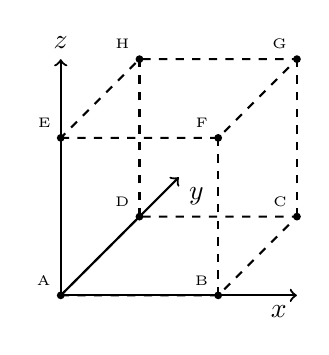
\begin{tikzpicture}[scale=1, x={(1cm,0cm)}, y={(0.5cm,0.5cm)}, z={(0cm,1cm)}]
  % Axes
  \draw[->, thick] (0,0,0) -- (3,0,0) node[anchor=north east] {\(x\)};
  \draw[->, thick] (0,0,0) -- (0,3,0) node[anchor=north west] {\(y\)};
  \draw[->, thick] (0,0,0) -- (0,0,3) node[anchor=south] {\(z\)};

  % Sommets
  \foreach \x/\y/\z/\name in {
    0/0/0/A, 2/0/0/B, 2/2/0/C, 0/2/0/D,
    0/0/2/E, 2/0/2/F, 2/2/2/G, 0/2/2/H}
    {
      \filldraw[black] (\x,\y,\z) circle (1pt) node[anchor=south east] {\tiny \name};
    }

  % Arêtes
  \draw[dashed] (0,0,0) -- (2,0,0) -- (2,2,0) -- (0,2,0) -- cycle;
  \draw[dashed] (0,0,2) -- (2,0,2) -- (2,2,2) -- (0,2,2) -- cycle;
  \draw[dashed] (0,0,0) -- (0,0,2);
  \draw[dashed] (2,0,0) -- (2,0,2);
  \draw[dashed] (2,2,0) -- (2,2,2);
  \draw[dashed] (0,2,0) -- (0,2,2);
\end{tikzpicture}
\end{minipage}
\begin{minipage}{0.45\textwidth}
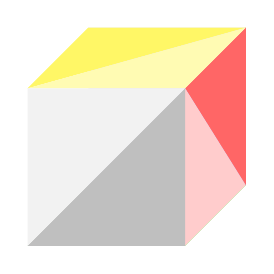
\begin{tikzpicture}[scale=1, line join=round]
  % Points du cube
  \coordinate (A) at (0,0,0);
  \coordinate (B) at (2,0,0);
  \coordinate (C) at (2,2,0);
  \coordinate (D) at (0,2,0);
  \coordinate (E) at (0,0,2);
  \coordinate (F) at (2,0,2);
  \coordinate (G) at (2,2,2);
  \coordinate (H) at (0,2,2);

  % Triangles - chaque face = 2 triangles
  \fill[blue!50]  (A) -- (B) -- (C) -- cycle;
  \fill[blue!10]  (A) -- (C) -- (D) -- cycle;

  \fill[green!60] (A) -- (B) -- (F) -- cycle;
  \fill[green!20] (A) -- (F) -- (E) -- cycle;

  \fill[red!60]   (B) -- (C) -- (G) -- cycle;
  \fill[red!20]   (B) -- (G) -- (F) -- cycle;

  \fill[yellow!60] (C) -- (D) -- (H) -- cycle;
  \fill[yellow!30] (C) -- (H) -- (G) -- cycle;

 % \fill[orange!50] (D) -- (A) -- (E) -- cycle;
 % \fill[orange!10] (D) -- (E) -- (H) -- cycle;

  \fill[gray!50]   (E) -- (F) -- (G) -- cycle;
  \fill[gray!10]   (E) -- (G) -- (H) -- cycle;

  % Arêtes
%  \draw[thick] (A) -- (B) -- (C) -- (D) -- cycle;
 % \draw[thick] (E) -- (F) -- (G) -- (H) -- cycle;
 % \draw[thick] (A) -- (E);
%  \draw[thick] (B) -- (F);
%  \draw[thick] (C) -- (G);
%  \draw[thick] (D) -- (H);
\end{tikzpicture}
\end{minipage}
\end{center}
\end{frame}

\begin{frame}[fragile]
  \frametitle{Le format \texttt{STL}}

  \begin{columns}
    \column{0.45\textwidth}
    \scriptsize
\begin{verbatim}
solid cube
  facet normal 0 0 1 // Face supérieure
    outer loop
      vertex 0 0 1
      vertex 1 0 1
      vertex 0 1 1
    endloop
  endfacet
  facet normal 0 0 1
    outer loop
      vertex 1 0 1
      vertex 1 1 1
      vertex 0 1 1
    endloop
  endfacet
  // Autres faces...
endsolid cube
\end{verbatim}
    \column{0.55\textwidth}
    \begin{figure}
      \centering
      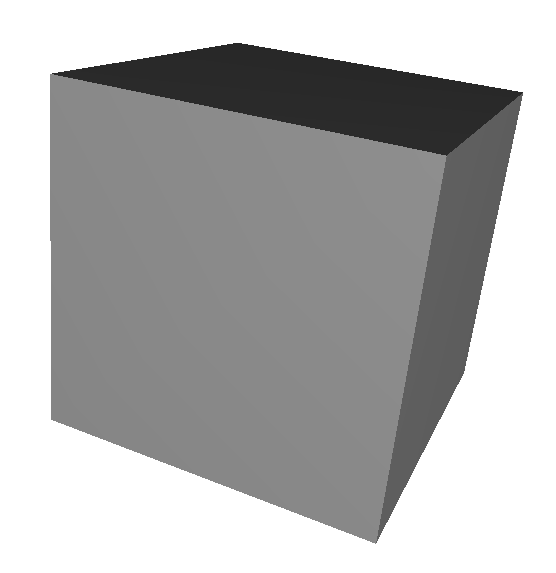
\includegraphics[width=3.5cm]{capture/cubestl.png} % Remplace par ton image
      \caption{\tiny fichier STL visualisé avec viewstl.com}
    \end{figure}
  \end{columns}
\end{frame}
